\documentclass[10pt,letterpaper]{article}
\usepackage[margin=0.82in]{geometry}
\usepackage[T1]{fontenc}
\usepackage{lmodern,microtype,amsmath,amssymb,booktabs,array}
\usepackage{xcolor,hyperref,fancyhdr,tikz}
\usetikzlibrary{arrows.meta,positioning}
\definecolor{navy}{HTML}{142A43}
\definecolor{teal}{HTML}{087E8B}
\definecolor{grayblue}{HTML}{EAF1F6}
\definecolor{muted}{HTML}{536779}
\hypersetup{colorlinks=true,linkcolor=teal,urlcolor=teal}
\pagestyle{fancy}\fancyhf{}\fancyhead[L]{\small\textcolor{muted}{SmolVLA / LIBERO}}\fancyhead[R]{\small\textcolor{muted}{Q10 critic and corrector}}\fancyfoot[C]{\small\thepage}\renewcommand{\headrulewidth}{0pt}
\setlength{\parindent}{0pt}\setlength{\parskip}{5pt}
\newcommand{\status}[1]{\textsf{\footnotesize\bfseries\color{teal}#1}}
\newcommand{\Q}{Q^{\pi}_{10}}
\begin{document}
\begin{flushleft}
{\Large\bfseries\color{navy} SmolVLA Q10 critic and corrector}\\[5pt]
{\large Pipeline, architecture, learning objective, and current evidence}\\[8pt]
{\small Technical snapshot \textbullet\ 27 September 2026 \textbullet\ repository commit \texttt{fea0a58}}
\end{flushleft}
\vspace{4pt}\color{teal}\rule{\linewidth}{1.2pt}\color{black}

\noindent\fcolorbox{teal}{grayblue}{\parbox{0.955\linewidth}{\textbf{Scope.} The current SmolVLA Q10 model is a \emph{critic}: it scores an already proposed ten-action chunk. Candidate reranking is the nearest-term \emph{corrector} experiment. The repository also contains an older, distinct PCP gradient corrector, which nudges a denoising estimate inside P\&P. These mechanisms must not be treated as a single validated system.}}

\section*{1. The quantity the critic should learn}
At a LIBERO decision boundary, let $x_t$ denote the observation, task instruction, robot state, and remaining episode budget. Let $A_t=(a_t,\ldots,a_{t+9})\in\mathbb R^{10\times 7}$ be the \emph{ten actions actually executed}. The target is the success probability after one intervention and a fixed continuation policy $\pi$:
\begin{equation}
\boxed{\Q(x_t,A_t)=\Pr\!\left(Y=1\mid x_t,\operatorname{do}(A_t),\text{then frozen SmolVLA P\&P }\pi\right).}
\end{equation}
Here $Y$ is binary terminal task success. The policy and its rollout procedure define the estimand: changing the continuation policy changes $Q$. This is \emph{policy evaluation} over candidate chunks, not an optimal-action $Q^*$ or a reward model for arbitrary actions.

For a recorded ten-step transition, the one-step Bellman target is
\begin{equation}
y_t=r_t+(1-d_t)\,\bar Q(x_{t+10},A^{\pi}_{t+10}), \qquad \gamma=1,
\end{equation}
where $r_t$ records success in that interval, $d_t$ is termination, and $A^{\pi}_{t+10}$ is the \emph{recorded} next chunk under frozen $\pi$. The target network $\bar Q$ is an exponential moving average. There is no $\max_A$: inserting one would train a different control objective. Remaining time belongs in $x_t$ because the task has a finite step limit.

\section*{2. Data-generation pipeline}
\begin{center}
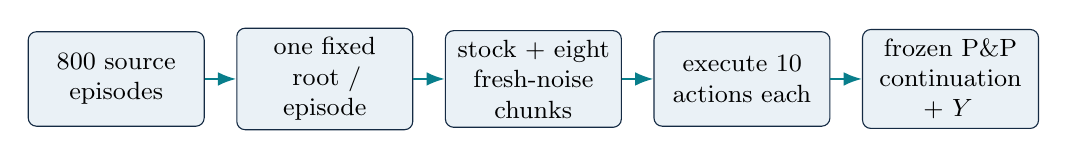
\begin{tikzpicture}[node distance=4mm, every node/.style={font=\small}, box/.style={draw=navy,rounded corners=3pt,fill=grayblue,align=center,minimum height=12mm,text width=0.165\linewidth}, arr/.style={-Latex,thick,draw=teal}]
\node[box] (src) {800 source\\episodes};
\node[box,right=of src] (root) {one fixed\\root / episode};
\node[box,right=of root] (prop) {stock + eight\\fresh-noise chunks};
\node[box,right=of prop] (fork) {execute 10\\actions each};
\node[box,right=of fork] (out) {frozen P\&P\\continuation + $Y$};
\draw[arr] (src)--(root);\draw[arr] (root)--(prop);\draw[arr] (prop)--(fork);\draw[arr] (fork)--(out);
\end{tikzpicture}
\end{center}
The source cohort contains 800 distinct episodes at indices 10--29. Root locations were fixed in an immutable manifest before the new candidate outcomes: 65\% were selected by a high $U_{10}$ uncertainty score, 35\% uniformly. The v4 fresh8 tree defines nine candidates at the \emph{same state}: the exact stored source chunk $A_0$, plus $A_1,\dots,A_8$ generated from fresh initial noise using P\&P. Each chunk is executed for ten actions; the same frozen P\&P continuation and future seed then produce an observed success/failure. Complete v3 roots can reuse their four existing fresh-noise branch artifacts; the remaining four are collected in v4. The four v3 perturbation-stream branches are excluded from v4.

The worker writes candidate metadata, chunk artifacts, observations, and continuations to Supabase. A separate snapshot/cache job validates complete trees and builds root records and ten-step transition windows. Roots and all nine branches stay together in an 80/20 train/validation split, stratified by suite and source outcome. \textbf{Unit of independent generalization: root state, not branch.} Nine correlated outcomes at one root are particularly valuable for same-state ranking, but 800 trees are 800 states, not 7,200 independent states.

\newpage
\section*{3. Architecture: one state and one candidate chunk in, one score out}
The critic is a \emph{separate} action-conditioned network. It receives cached SmolVLA context and an already generated $10\times7$ chunk; it does not run the VLA action generator during critic training. Two token streams meet in a Transformer decoder:

\begin{center}
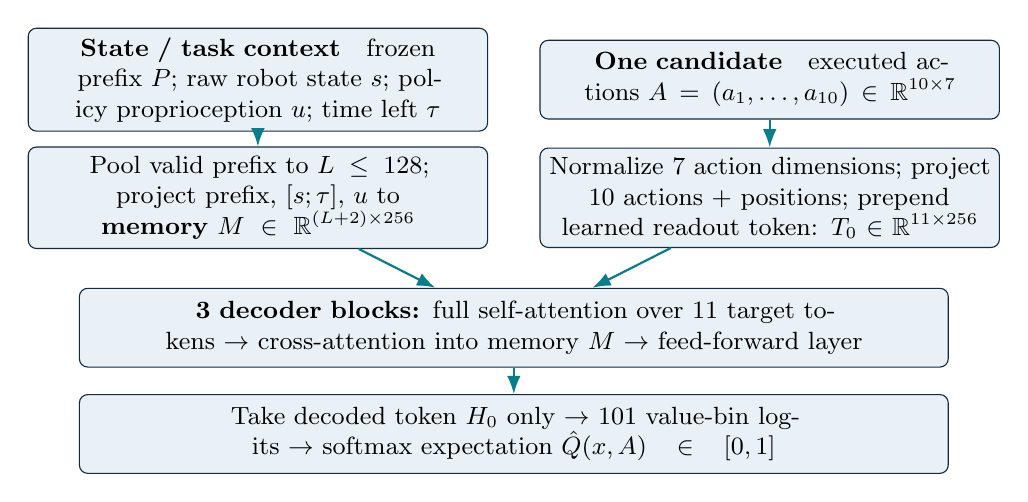
\begin{tikzpicture}[node distance=5mm, every node/.style={font=\small}, box/.style={draw=navy,rounded corners=3pt,fill=grayblue,align=center,minimum height=10mm}, arr/.style={-Latex,thick,draw=teal}]
\node[box,text width=5.6cm] (ctx) at (-3.25,2.15) {\textbf{State / task context}\quad frozen prefix $P$; raw robot state $s$; policy proprioception $u$; time left $\tau$};
\node[box,text width=5.6cm] (act) at (3.25,2.15) {\textbf{One candidate}\quad executed actions $A=(a_1,\ldots,a_{10})\in\mathbb R^{10\times7}$};
\node[box,text width=5.6cm] (mem) at (-3.25,0.65) {Pool valid prefix to $L\leq128$; project prefix, $[s;\tau]$, $u$ to \textbf{memory} $M\in\mathbb R^{(L+2)\times256}$};
\node[box,text width=5.6cm] (tgt) at (3.25,0.65) {Normalize 7 action dimensions; project 10 actions + positions; prepend learned readout token: $T_0\in\mathbb R^{11\times256}$};
\node[box,text width=10.8cm] (dec) at (0,-1.0) {\textbf{3 decoder blocks:} full self-attention over 11 target tokens $\rightarrow$ cross-attention into memory $M$ $\rightarrow$ feed-forward layer};
\node[box,text width=10.8cm] (head) at (0,-2.35) {Take decoded token $H_0$ only $\rightarrow$ 101 value-bin logits $\rightarrow$ softmax expectation $\hat Q(x,A)\in[0,1]$};
\draw[arr] (ctx)--(mem);\draw[arr] (act)--(tgt);\draw[arr] (mem)--(dec);\draw[arr] (tgt)--(dec);\draw[arr] (dec)--(head);
\end{tikzpicture}
\end{center}

\textbf{Context stream.} $P\in\mathbb R^{L_0\times d_p}$ is the stored visual/language prefix embedding at this decision boundary, with a validity mask. Valid tokens are kept in order; if $L_0>128$, adaptive average pooling compresses them to 128. Each pooled token passes through a learned layer norm and linear projection to width 256. The raw robot vector augmented with remaining episode fraction, $[s;\tau]$, and the SmolVLA policy proprioception vector $u$ each receive their \emph{own} learned norm/linear projection and are appended as two memory tokens. Thus, schematically,
\begin{equation}
M=[\phi_P(\widetilde P_1),\ldots,\phi_P(\widetilde P_L),\phi_s([s;\tau]),\phi_u(u)]
\in\mathbb R^{(L+2)\times256}.
\end{equation}
The upstream SmolVLA features are frozen/cached; these three critic-side projections \emph{are trained}. The raw robot state and policy proprioception are separate inputs even if some information overlaps.

\textbf{Action stream and readout.} Action means $\mu\in\mathbb R^7$ and standard deviations $\sigma\in\mathbb R^7$ are fitted on training-root candidates only. For action position $i$, $e_i=\operatorname{LN}(W_a((a_i-\mu)/\sigma)+b_a)+p_i$, where $p_i$ is a learned position vector. A learned vector $c_{\rm RL}$ is prepended: $T_0=[c_{\rm RL},e_1,\ldots,e_{10}]$. The ``RL token'' is simply a learned \emph{readout slot}, analogous to a classification token; it is not an extra reward observation or a separate RL policy. There is no causal target mask: in each of the three decoder layers it can attend to all ten candidate actions, while cross-attention reads the state/task memory. The final prediction uses only that token:
\begin{equation}
H=D_\theta^{(3)}(T_0;M),\qquad z=W_vH_0+b_v,\qquad
\hat Q(x,A)=\sum_{k=0}^{100}\frac{k}{100}\operatorname{softmax}(z)_k.
\end{equation}
The decoder has width 256, 8 heads, FFN width 1024, and dropout 0.20; with a 512-wide prefix, the critic has about 3.33 million trainable parameters. For nine candidates at one root, the code repeats the \emph{same} context nine times and scores each chunk independently: candidates do not attend to one another. The 101-bin output is a modeling choice, not evidence of 101 observed return values; root outcomes are binary.

\newpage
\section*{4. Two training arms on one immutable snapshot}
\textbf{Root Monte Carlo (MC).} For each root $j$ and candidate $i$, the full continuation gives $Y_{ji}\in\{0,1\}$. The implemented loss applies binary cross-entropy to the \emph{expected value} of the 101-bin head:
\begin{equation}
\mathcal L_{\rm MC}=-\frac{1}{9B}\sum_{j=1}^{B}\sum_{i=0}^{8}\left[Y_{ji}\log\hat q_{ji}+(1-Y_{ji})\log(1-\hat q_{ji})\right].
\end{equation}
Training samples roots and evaluates all nine same-state candidates. This directly supervises the proposed intervention but each label reflects one continuation random stream.

\textbf{Tree temporal difference (TD).} The cache provides ten-action windows through the branch continuation. The implemented target is $y_t=\operatorname{clip}_{[0,1]}\{r_t+(1-d_t)\bar q_{t+10}\}$. The scalar $y_t$ is spread over nearby value bins using a narrow Gaussian target $h_k(y_t)$, followed by categorical cross-entropy:
\begin{equation}
\mathcal L_{\rm TD}=-\frac1B\sum_t\sum_{k=0}^{100}h_k(y_t)\log p_{\theta,k}(x_t,A_t),\quad
\bar\theta\leftarrow(1-0.005)\bar\theta+0.005\theta.
\end{equation}
TD uses more boundaries, but bootstraps and may spend most updates on downstream continuation actions rather than fork choices. A single sigmoid head with BCE against $Y$ for MC or soft target $y_t\in[0,1]$ for TD is a clean, \emph{not-yet-run} ablation. Both forms seek a success probability; the bins are not required by the Bellman equation.

Both arms currently use AdamW ($10^{-4}$ initial learning rate, cosine schedule, 100 warmup updates), batch size 8 roots for MC or 8 sampled TD branches with 8 windows each, 2,000 updates, gradient clipping at 1, and periodic held-out evaluation. Q training runs on cached features and does not require running SmolVLA or LIBERO on the training GPU.

\section*{5. What ``corrector'' means here}
\textbf{Proposed, conservative candidate selector.} At deployment, generate $A_0$ (stock) and fresh P\&P candidates $A_1,\dots,A_8$ at one observation, then score them with $\hat Q$. A stock-preserving rule is
\begin{equation}
i^*=\arg\max_{i\ge1}\hat Q(x,A_i),\qquad
A_{\rm chosen}=\begin{cases}A_{i^*},&\hat Q(x,A_{i^*})-\hat Q(x,A_0)>\tau,\\A_0,&\text{otherwise.}\end{cases}
\end{equation}
The threshold $\tau$ must be tuned on a separate development set and evaluated on fresh roots. This rule \emph{selects} an already generated on-distribution chunk. It does not modify the chunk. A future action optimizer could maximize $\hat Q(x,A)-\lambda\lVert A-A_0\rVert^2$, possibly with P\&P projection, but it risks exploiting errors off the training distribution and needs new simulator evaluations.

\textbf{Historical PCP gradient corrector.} The separate \texttt{pnp/pcp.py} path has a three-layer residual MLP over a flattened denoising estimate, observation embedding, and chunk-position/noise-level features. When its calibrated success score falls below a gate, it applies $z' = z+\lambda\nabla_z\hat Q_{\rm PCP}$, then re-noises the result within P\&P. This is an actual action-changing corrector, but it is \emph{not} the current SmolVLA Q10 transformer, its training data, or a validated consequence of the fresh8 experiment.

\newpage
\section*{6. Results, limits, and immediate decision}
On the completed \textbf{v3 480-tree snapshot} (384 training roots, 96 held-out roots; original + four fresh + four perturbation candidates), stock succeeded on 66/96 validation roots; an oracle over recorded candidates would succeed on 74/96. After 2,000 updates, ungated root-MC argmax selected 60/96 (0 rescues, 6 spoils; within-root pair accuracy 0.562). TD argmax selected 56/96 (2 rescues, 12 spoils; pair accuracy 0.475). Thus the observed critic-based argmax \emph{degraded} success in this holdout. These results do not yet establish a useful deployed corrector.

The intended \textbf{v4 fresh8} experiment has 800 possible roots and nine fresh-only candidates per root; the code and three Colab workers exist. The three one-tree smoke runs shown in the conversation completed successfully, but they are not evidence that all 800 trees are complete. Freeze a complete v4 snapshot before training and report its actual root count. Then use nested training-root subsets with a fixed validation set to measure scaling. Evaluate stock, oracle, selected success, rescues, spoils, mixed-root pair accuracy, calibration, and per-suite effects. Reserve unseen episode indices for a final test; the existing 10--29 cohort and single future seed per branch limit external validity.

\section*{7. Interpretation and next controlled comparisons}
The central test is whether the model can \emph{rank actions at the same root}, not merely predict whether a task or scene is easy. An observation-only shortcut can achieve useful calibration while failing to order the nine candidates. Report a within-root pair metric only on mixed roots, and compare selection to the stock action at each identical root.

The controlled comparisons are: (i) nested 100/200/400/$\sim$640 training roots with one fixed holdout, (ii) the 101-bin decoder against a scalar sigmoid and a smaller action-conditioned head, (iii) root MC against TD with root-balanced window sampling, and (iv) stock-only, ungated argmax, and a threshold tuned away from the final test. Change one factor at a time.
For a genuine action-changing corrector, score improvement on \emph{newly generated and executed} chunks. Offline selection within the recorded nine candidates cannot establish that gradient ascent in action space remains on the policy's support. Conversely, the fresh8 candidates directly match the P\&P proposal distribution the selector would encounter, which is why they are the clean first test.

{\small\textbf{Repository basis.} \texttt{pnp/smolvla\_fresh8\_collection.py}; \texttt{pnp/smolvla\_tree\_bellman\_finetune.py};\\
\texttt{pnp/qplanning\_critic/model.py}; \texttt{pnp/smolvla\_success\_critic.py}; \texttt{pnp/pcp.py};\\
\texttt{SMOLVLA\_Q10\_DIAGNOSIS\_2026-09-26.md}. Status and results reflect this repository snapshot and its documented Modal run; this report did not perform a new training run.}
\end{document}
